% !TeX program = pdflatex
% !TeX encoding = UTF-8
% Compilar en TeXstudio: F6 (pdflatex) dos veces
% Estilo IEEE (como el artículo de Duarte, 2026): Times, carta, dos columnas,
% secciones en números romanos y referencias numéricas [1].
\documentclass[10pt,letterpaper,twocolumn]{article}
\usepackage[english,spanish,es-noquoting,es-tabla,es-nodecimaldot]{babel}
\usepackage[T1]{fontenc}
\usepackage{times}            % texto en Times (matemáticas en Computer Modern, como en IEEE)

\usepackage[
  letterpaper,
  top=0.75in, bottom=1in,
  left=0.625in, right=0.625in,
  columnsep=0.25in,
  headheight=15pt, headsep=10pt
]{geometry}

\usepackage[dvipsnames]{xcolor}
\usepackage{graphicx}
\usepackage{amsmath}
\usepackage{amssymb}
\usepackage{array}
\usepackage{tabularx}
\usepackage{booktabs}
\usepackage{multirow}
\usepackage{enumitem}
\setlist{leftmargin=*, itemsep=1pt, topsep=3pt}
\usepackage{csquotes}
\usepackage{stfloats}         % permite figuras anchas [b] al pie de página

%%% Referencias numéricas [1] %%%
\usepackage[numbers,square,sort&compress]{natbib}
\setlength{\bibsep}{2pt}
\newcommand{\parencite}{\citep}

%%% Títulos de sección estilo IEEE %%%
\usepackage{titlesec}
\renewcommand{\thesection}{\Roman{section}}
\renewcommand{\thesubsection}{\thesection-\Alph{subsection}}
\titleformat{\section}{\centering\normalfont\scshape}{\thesection.}{0.5em}{}
\titleformat{\subsection}{\normalfont\itshape}{\thesubsection.}{0.5em}{}
\titlespacing*{\section}{0pt}{12pt plus 2pt}{6pt}
\titlespacing*{\subsection}{0pt}{8pt plus 2pt}{4pt}

%%% Títulos de figuras y tablas %%%
\usepackage{caption}
\captionsetup{font=small, labelsep=colon, hypcap=false}
\renewcommand{\thetable}{\Roman{table}}
\captionsetup[table]{name=TABLA}
\captionsetup[figure]{name=Figura}

%%% Encabezados %%%
\usepackage{fancyhdr}
\pagestyle{fancy}
\fancyhf{}
\fancyhead[L]{Jesús Molina, John González, Julián Bernal}
\fancyhead[R]{\leftmark}
\fancyfoot[C]{\thepage}
\renewcommand{\headrulewidth}{0.4pt}
\renewcommand{\sectionmark}[1]{\markboth{\thesection}{\thesection}}

% Primera página: membrete de la especialización y logo
\fancypagestyle{primera}{
  \fancyhf{}
  \renewcommand{\headrulewidth}{0pt}
  \fancyhead[L]{\begin{tabular}[b]{|l}
    \textcolor{PineGreen}{\textbf{Especialización}}\\
    \textcolor{PineGreen}{\textbf{en Estadística Aplicada}}\\
    \textcolor{PineGreen}{Facultad de Ingeniería y Ciencias Básicas}
  \end{tabular}}
  \fancyhead[R]{
\includegraphics[width=2cm]{img/logoFULL.png}}
  \fancyfoot[C]{\thepage}
}

% hyperref al final del preámbulo
\usepackage{hyperref}
\urlstyle{same}
\hypersetup{colorlinks=true, linkcolor=black, citecolor=black, urlcolor=black}

%%% Bloque de autor estilo IEEE %%%
\newcommand{\autor}[2]{%
  \begin{tabular}[t]{c}
    {\large #1}\\[1pt]
    \small #2
  \end{tabular}}

\begin{document}

%==================  TÍTULO Y AUTORES (a todo el ancho)
\twocolumn[{%
\thispagestyle{primera}
\vspace*{2.2cm}
\begin{center}
{\fontsize{20}{24}\selectfont
¿Pueden los simulacros de una empresa externa anticipar el resultado de la Saber 11°? Modelo predictivo y regla de priorización para una institución educativa del Atlántico\\[2pt]
Can an External Company's Mock Tests Anticipate Saber 11° Results? A Predictive Model and Prioritization Rule for a School in Atlántico\par}
\vspace{16pt}
\autor{Jesús Molina Cantillo}{Estudiante, Facultad de Ingeniería y Ciencias Básicas\\ Fundación Universitaria Los Libertadores}
\hspace{1.5cm}
\autor{John González Veloza}{Profesor, Facultad de Ingeniería y Ciencias Básicas\\ Fundación Universitaria Los Libertadores\\ Bogotá, Colombia}
\\[10pt]
\autor{Julián Bernal Salamanca}{Profesor, Facultad de Ingeniería y Ciencias Básicas\\ Fundación Universitaria Los Libertadores\\ Bogotá, Colombia}
\end{center}
\vspace{14pt}
}]

%==================  RESUMEN Y ABSTRACT (en la primera columna, negrilla, como IEEE)
{\fontsize{9}{10.5}\selectfont\bfseries
\noindent\textit{Resumen}---Contexto: En las cohortes 2025 y 2026, la Institución Educativa Técnica Agrícola (I.E.T.A.) Juan Domínguez Romero de Caracolí (Malambo, Atlántico) estableció convenios con una empresa externa para preparar a sus estudiantes para la prueba Saber~11°. La preparación consistió en dos simulacros (S1 y S2) aplicados antes de la prueba oficial, y con sus resultados la institución decidió a quién reforzar. Propósito: Esta investigación evaluó si esa información servía para anticipar el puntaje global oficial (SB11\_GLOBAL, escala 0--500) y para identificar a tiempo a los estudiantes que terminarían en el cuartil inferior de su promoción. Metodología: Con los 97 estudiantes que presentaron las tres pruebas, se entrenaron modelos con la cohorte 2025 (Train, \textit{n}~=~45) y se evaluaron con la cohorte 2026 (Test, \textit{n}~=~52), que no intervino en el ajuste. Resultados: Una regresión lineal con el promedio de S1 y S2 redujo el error medio absoluto de 27,7 puntos (línea base) a 18,1 (IC 95\,\%: 14,6--21,7). Una regresión logística con la misma variable alcanzó en Test un AUC de 0,87 (IC 95\,\%: 0,77--0,95), una sensibilidad de 1,00 (IC 95\,\%: 0,75--1,00) y una exactitud balanceada de 0,83 en el umbral elegido. Frente a la regla que usaba la empresa (nivel I/1), el modelo cometió menos errores de clasificación (prueba exacta de McNemar, \textit{p}~=~0,004) y elevó la especificidad de 0,49 a 0,67. Los modelos más complejos no mejoraron estos resultados y mostraron sobreajuste. Conclusiones: El estudio produjo una regla de tres prioridades (alta, media y baja), aplicable con solo el promedio de los dos simulacros.

\textit{Palabras clave}---Saber 11°, simulacros, aprendizaje automático, alerta temprana, validación temporal.

\begin{otherlanguage}{english}
	\textit{Abstract}---Context: For the 2025 and 2026 cohorts, the Institución Educativa Técnica Agrícola (I.E.T.A.) Juan Domínguez Romero school in Caracolí (Malambo, Atlántico) entered into agreements with an external company to prepare its students for the Saber~11° exam. This preparation consisted of two mock tests (S1 and S2) administered before the official exam, and the school used their results to decide which students would receive extra support. Purpose: This research assessed whether that information could anticipate the official global score (SB11\_GLOBAL, 0--500 scale) and identify, in time, the students who would end up in the bottom quartile of their cohort. Methodology: Using the 97 students who sat all three tests, models were trained on the 2025 cohort (Train, \textit{n}~=~45) and evaluated on the 2026 cohort (Test, \textit{n}~=~52), which was not used for fitting. Results: A linear regression on the average of S1 and S2 reduced the mean absolute error from 27.7 points (baseline) to 18.1 (95\,\% CI: 14.6--21.7). A logistic regression on the same variable reached, on Test, an AUC of 0.87 (95\,\% CI: 0.77--0.95), a sensitivity of 1.00 (95\,\% CI: 0.75--1.00) and a balanced accuracy of 0.83 at the chosen threshold. Compared with the rule used by the company (level I/1), the model made fewer classification errors (exact McNemar test, \textit{p}~=~0.004) and raised specificity from 0.49 to 0.67. More complex models did not improve these results and showed overfitting. Conclusions: The study produced a three-level priority rule (high, medium and low) that can be applied using only the average of the two mock tests.
	
	\textit{Index Terms}---Saber 11°, mock tests, machine learning, early warning, temporal validation.
\end{otherlanguage}
\par}

%==================  INTRODUCCIÓN
\section{Introducción}

La prueba Saber~11° resume el aprendizaje de la educación media en un puntaje global de 0 a 500, en el que Lectura crítica, Matemáticas, Sociales y ciudadanas y Ciencias naturales pesan tres veces más que Inglés \parencite{icfes2026saber11}. Por el peso que tiene en el acceso a la educación superior, muchas instituciones contratan simulacros con el formato del examen. Practicar con pruebas mejora la retención \parencite{roediger2006test}, pero eso no garantiza que el puntaje del simulacro sea una buena señal del resultado oficial.

Esa segunda función, la de anticipar, es la que interesa aquí. La minería de datos educativos ha mostrado que los registros que una institución ya tiene permiten predecir el desempeño y actuar antes \parencite{romero2020educational}, siempre que se defina con precisión qué se predice y cómo se valida \parencite{alyahyan2020predicting}. En Colombia, Timarán-Pereira et~al. \parencite{timaran2019arboles} aplicaron árboles de decisión a un repositorio de resultados de Saber~11° para identificar patrones asociados al buen o mal desempeño de estudiantes de bachillerato. Un sistema de alerta, además, solo es útil si acierta con quienes necesitan apoyo y no marca en exceso a quienes no lo necesitan \parencite{bowers2013dropout}.

En la I.E.T.A. Juan Domínguez Romero de Caracolí, la empresa entrega con cada simulacro un nivel de desempeño (I/1, M/2 o S/3). Hasta ahora nadie había comprobado si esos puntajes y niveles anticipan bien el resultado oficial. Este documento responde dos preguntas: (1) ¿qué tan bien estiman los simulacros el puntaje global de Saber~11°?, y (2) ¿qué regla de decisión permite a la institución priorizar el refuerzo con menos errores que la clasificación de la empresa? El objetivo es construir y validar, con datos de la propia institución, un modelo que responda ambas preguntas y que pueda traducirse en una regla de decisión aplicable por el colegio. La variable objetivo es SB11\_GLOBAL.

%==================  DATOS
\section{Datos y síntesis del análisis exploratorio}

Se usaron las bases de modelado anonimizadas de 2025 y 2026, con una fila por estudiante y tres mediciones en orden temporal: S1, S2 y Saber~11°. El análisis principal incluye los 97 estudiantes con las tres pruebas observadas; los 15 que faltaron a un simulacro se reservaron para un análisis de sensibilidad. De todo el análisis exploratorio se seleccionaron tres gráficos, porque son los que explican las decisiones del modelo.

\begin{figure*}[!t]
    \centering
    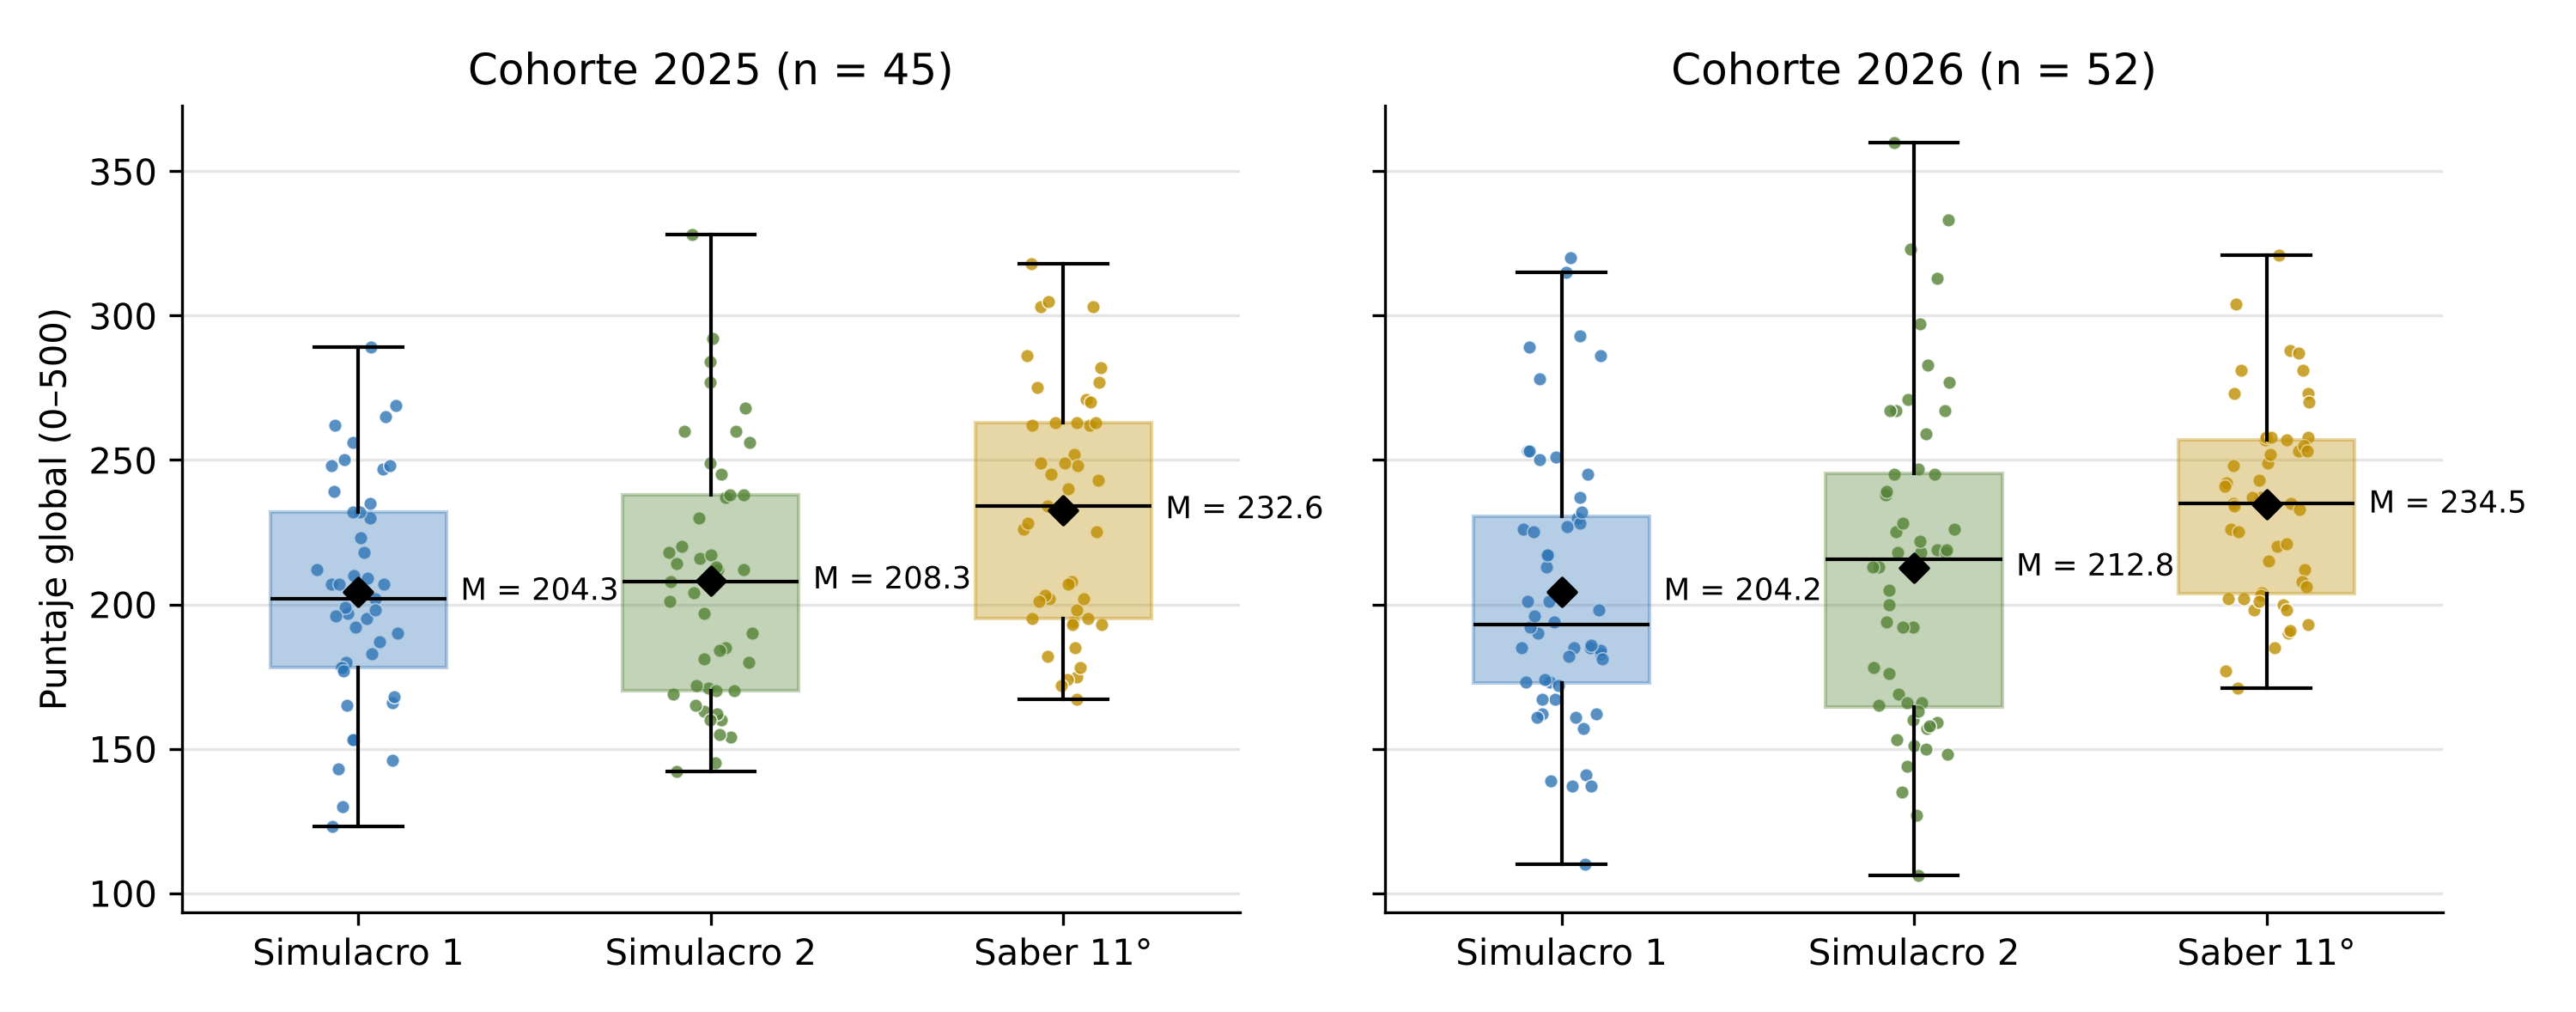
\includegraphics[width=0.9\textwidth]{img/fig1_distribucion_cohortes.png}
    \caption{Distribución del puntaje global por prueba y cohorte (el rombo indica la media).}
    \label{fig:distribucion}
\end{figure*}

\textit{La variable objetivo y la necesidad de calibrar.} La figura~\ref{fig:distribucion} muestra dos hechos. Primero, SB11\_GLOBAL tiene una distribución casi simétrica y medias muy parecidas en las dos cohortes (232,6 y 234,5; \textit{t} de Welch~=~$-0{,}25$, \textit{p}~=~0,80), lo que permite entrenar con un año y evaluar con el otro. Segundo, los simulacros quedan entre 22 y 30 puntos por debajo del resultado oficial. Por eso el puntaje bruto del simulacro no puede usarse como estimación: hace falta un modelo que lo calibre.

\begin{figure}[!t]
    \centering
    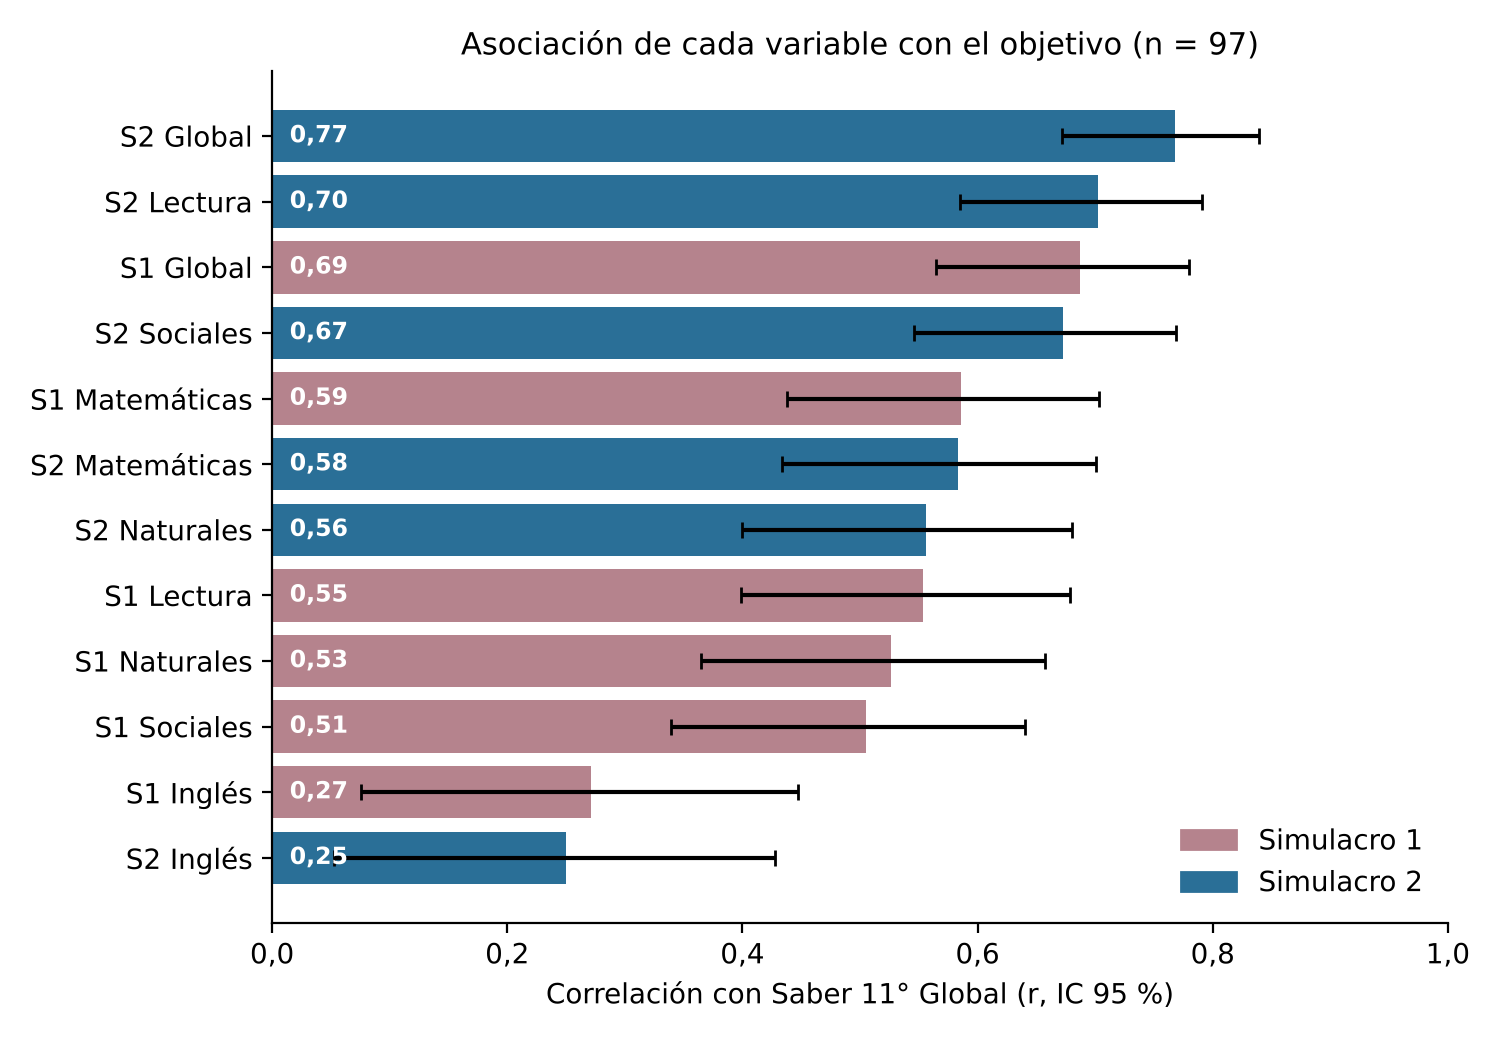
\includegraphics[width=\columnwidth]{img/fig2_correlacion_objetivo.png}
    \caption{Correlación de cada variable con SB11\_GLOBAL e intervalos de confianza del 95\,\% (\textit{n}~=~97).}
    \label{fig:correlacion}
\end{figure}

\textit{Qué predictores usar.} En la figura~\ref{fig:correlacion}, S2 Global (\textit{r}~=~0,77) y S1 Global (\textit{r}~=~0,69) son las variables más asociadas con el objetivo; Inglés es la más débil en ambos simulacros (\textit{r}~$\approx$~0,25). S1 y S2 están relacionados (\textit{r}~=~0,64 con las dos cohortes juntas), pero no son redundantes, y su promedio alcanza \textit{r}~=~0,81. Esto justifica dos familias de modelos: una sencilla, con el promedio de S1 y S2, y otra con las diez áreas por separado, para comprobar si el detalle por área añade algo.

\begin{figure}[!t]
    \centering
    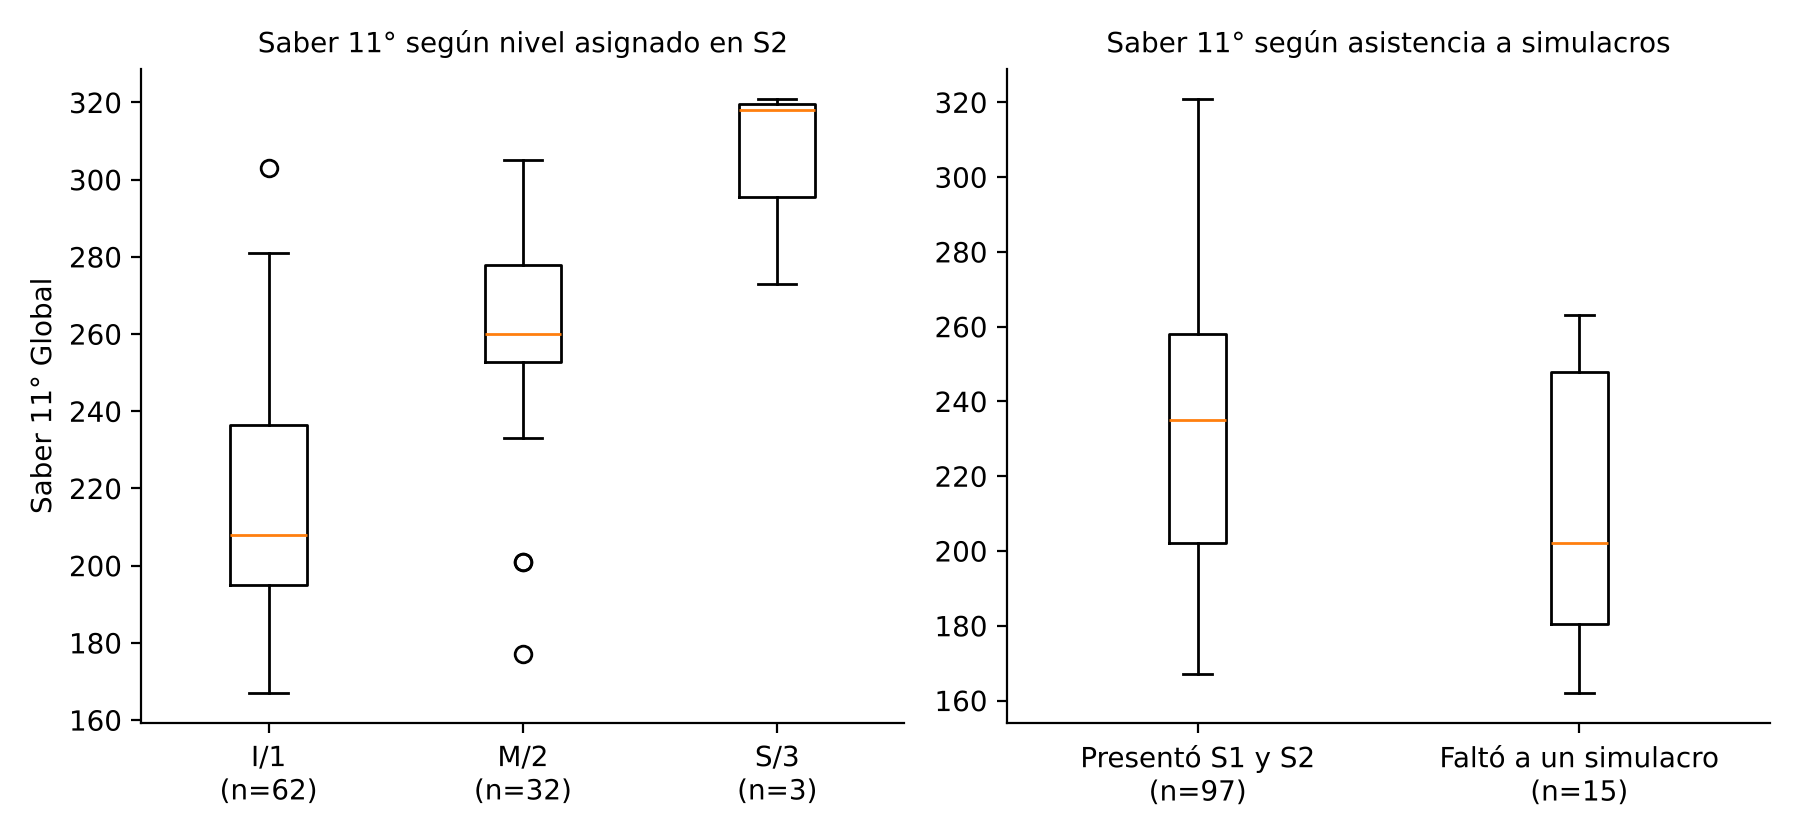
\includegraphics[width=\columnwidth]{img/fig3_nivel_asistencia.png}
    \caption{SB11\_GLOBAL según el nivel asignado por la empresa en S2 y según la asistencia a los simulacros.}
    \label{fig:nivel}
\end{figure}

\textit{La regla actual y la tarea de clasificación.} La figura~\ref{fig:nivel} muestra que los niveles de la empresa ordenan a los estudiantes, pero el nivel I/1 agrupa a casi dos de cada tres y mezcla puntajes oficiales de 167 a 303. Esa clasificación es la regla experta que el modelo debe superar. También muestra que quienes faltaron a un simulacro obtuvieron 23 puntos menos (\textit{d}~=~$-0{,}62$), por lo que la inasistencia se trata como una alerta adicional y no se borra del análisis.

\textit{Consideraciones éticas.} El tratamiento de los datos se ajustó a la Ley Estatutaria 1581 de 2012 sobre protección de datos personales \parencite{ley1581}, en particular a sus principios de finalidad, acceso y circulación restringida, seguridad y confidencialidad. Como la mayoría de los estudiantes de grado 11° son menores de edad, se atendió además la protección reforzada que esa ley establece para los datos de niños, niñas y adolescentes. Los nombres se reemplazaron por códigos (E001, E002, \ldots) antes del análisis; la tabla que vincula códigos y nombres quedó bajo custodia de la institución y no se distribuyó. Los resultados se informan solo de forma agregada y ningún dato individual se publica. El rector de la institución avaló el uso de los datos en esta investigación, con la condición de que no apareciera el nombre de ningún estudiante; por eso las bases que acompañan el artículo solo contienen códigos.

%==================  METODOLOGÍA
\section{Metodología}

\subsection{Tareas de predicción}

Se plantearon dos tareas supervisadas sobre la misma base. En la regresión, el objetivo es SB11\_GLOBAL. En la clasificación, el objetivo es si el estudiante queda en el cuartil inferior de Saber~11° de su propia cohorte (riesgo~=~1). Se eligió una definición relativa para que la etiqueta señale, en cada promoción, al grupo de menor desempeño y mantenga una prevalencia estable entre cohortes. El cuartil define quién está en riesgo, no cuántos estudiantes reciben apoyo: ese número lo determina el umbral de decisión, que favorece la sensibilidad porque omitir a un estudiante en riesgo se considera más costoso que reforzar a uno que no lo necesitaba (Anexo~B). Por eso el grupo con refuerzo resulta mayor que el cuartil. La prevalencia de la clase positiva es del 26,7\,\% en Train y del 25,0\,\% en Test.

\subsection{Separación de los datos}

La división fue temporal: Train~=~cohorte 2025 (\textit{n}~=~45; 46,4\,\%) y Test~=~cohorte 2026 (\textit{n}~=~52; 53,6\,\%). Se prefirió a una partición aleatoria porque reproduce el uso real del modelo (aprender con una promoción y aplicarlo a la siguiente) y evita que estudiantes de un mismo año queden repartidos entre entrenamiento y prueba \parencite{hastie2009elements,kaufman2012leakage}. El conjunto Test solo se usó para la evaluación final. Dentro de Train:

\begin{itemize}
    \item los hiperparámetros se ajustaron con validación cruzada repetida (5 pliegues $\times$ 3 repeticiones; estratificada en clasificación);
    \item los umbrales de decisión se eligieron con probabilidades fuera de pliegue (validación cruzada estratificada de 5 pliegues), sin mirar Test.
\end{itemize}

Como comprobaciones de robustez se repitió el análisis en sentido inverso (Train 2026~$\rightarrow$~Test 2025) y se incluyeron los 15 estudiantes con un simulacro faltante (Train \textit{n}~=~57, Test \textit{n}~=~55).

\subsection{Algoritmos}

Todos los modelos se implementaron en Python con scikit-learn \parencite{pedregosa2011scikit}, dentro de \textit{pipelines} que encadenan la imputación, el escalado y el modelo (tabla~\ref{tb:algoritmos}).

\begin{table}[!t]
\centering
\footnotesize
\renewcommand{\arraystretch}{1.15}
\begin{tabularx}{\columnwidth}{@{}l l >{\raggedright\arraybackslash}X@{}}
\toprule
\textbf{Tarea} & \textbf{Modelo} & \textbf{Predictores e hiperparámetros} \\
\midrule
\multirow{5}{*}{Regresión}
 & Línea base & Media de SB11\_GLOBAL en Train \\
 & Regla experta & Puntaje bruto de S2 como estimación \\
 & Regresión lineal & Promedio de S1 y S2 \\
 & Ridge & 10 áreas estandarizadas; $\alpha$ entre $10^{-2}$ y $10^{3}$ por validación cruzada \parencite{hastie2009elements} \\
 & Random Forest & 10 áreas; 200 árboles; profundidad $\in$ \{2, 3, sin límite\}; hoja mínima $\in$ \{1, 5\} \parencite{breiman2001random} \\
\midrule
\multirow{5}{*}{\shortstack[l]{Clasifi-\\cación}}
 & Línea base & Clase mayoritaria (nadie en riesgo) \\
 & Regla experta & Nivel I/1 asignado por la empresa en S2 \\
 & Logística & Promedio de S1 y S2 estandarizado \\
 & Logística L2 & 10 áreas estandarizadas; $C$ entre $10^{-2}$ y $10^{2}$ \\
 & Random Forest & 10 áreas; clases balanceadas; misma rejilla que en regresión \\
\bottomrule
\end{tabularx}
\caption{Algoritmos comparados.}
\label{tb:algoritmos}
\end{table}

\subsection{Métricas}

En regresión se reportan el error medio absoluto (MAE, en puntos de la escala), la raíz del error cuadrático medio (RMSE) y $R^2$. En clasificación, como la clase positiva es minoritaria, la exactitud (\textit{accuracy}) no se usa para elegir el modelo: un clasificador que declara a todos \enquote{sin riesgo} obtiene 0,75 sin detectar a nadie. Se usan el área bajo la curva ROC \parencite{fawcett2006roc}, el área bajo la curva precisión--sensibilidad, más informativa con clases desbalanceadas \parencite{saito2015precision}, la exactitud balanceada, la sensibilidad, la especificidad, la precisión y F1. En regresión, un modelo complejo solo se prefiere si mejora al lineal en al menos dos puntos de MAE en ambos sentidos de validación y no muestra sobreajuste. En clasificación, los modelos se compararon en este orden: primero, la sensibilidad en el umbral de decisión, porque omitir a un estudiante en riesgo es el error más costoso; después, la exactitud balanceada; y, por último, la estabilidad, medida por la brecha entre Train y Test y por el desempeño al invertir los años. Ante resultados equivalentes, se prefirió el modelo más sencillo. La incertidumbre se cuantificó con intervalos de confianza del 95\,\% de Clopper--Pearson para la sensibilidad y la especificidad \parencite{clopper1934}, y con \textit{bootstrap} percentil (2000 remuestreos de Test) para el MAE y el AUC \parencite{efron1993}. La comparación con la regla de la empresa, hecha sobre los mismos estudiantes, se evaluó con la prueba exacta de McNemar \parencite{mcnemar1947}.

\subsection{Interpretabilidad}

Para entender qué impulsa las predicciones se usaron tres recursos: los coeficientes del modelo lineal y de la regresión logística, con sus intervalos de confianza y valores \textit{p}, estimados en Train sin penalización; los coeficientes de Ridge con las diez áreas estandarizadas, que indican el peso de cada área; y la traducción de los umbrales de probabilidad a valores del promedio de los simulacros, que convierte el modelo en una regla explícita.
El código, las bases anonimizadas y la herramienta de priorización están disponibles en \url{https://github.com/uajesusmc/prediccion-saber11-simulacros}.

%==================  RESULTADOS
\section{Resultados}

\subsection{Comparación de modelos}

\begin{table*}[!t]
\centering
\small
\begin{tabular}{@{}lccccc@{}}
\toprule
\textbf{Modelo} & \textbf{MAE} & \textbf{AUC} & \textbf{Sensibilidad [IC 95\,\%]} & \textbf{Especificidad [IC 95\,\%]} & \textbf{Exact. balanceada} \\
\midrule
Línea base & 27,7 & 0,50 & 0,00 [0,00; 0,25] & 1,00 [0,91; 1,00] & 0,50 \\
Regla experta (empresa) & 33,5 & 0,67 & 0,85 [0,55; 0,98] & 0,49 [0,32; 0,65] & 0,67 \\
Promedio S1-S2 (lineal / logística) & 18,1 & 0,87 & 1,00 [0,75; 1,00] & 0,67 [0,50; 0,81] & 0,83 \\
10 áreas (Ridge / logística L2) & 16,4 & 0,87 & 0,92 [0,64; 1,00] & 0,69 [0,52; 0,83] & 0,81 \\
Random Forest $\cdot$ 10 áreas & 15,2 & 0,87 & 0,77 [0,46; 0,95] & 0,72 [0,55; 0,85] & 0,74 \\
\bottomrule
\end{tabular}
\caption{Resultados principales en Test (cohorte 2026, \textit{n}~=~52; 13 estudiantes en riesgo y 39 sin riesgo). Intervalos de Clopper--Pearson. El detalle de Train y Test está en el Anexo~C.}
\label{tb:resultados}
\end{table*}

Los tres modelos entrenados superan con claridad a la línea base y a la regla experta (tabla~\ref{tb:resultados}). Usar el puntaje bruto de S2 como estimación es incluso peor que predecir la media (MAE de 33,5 frente a 27,7), lo que confirma que los simulacros deben calibrarse. Los tres modelos entrenados alcanzan el mismo AUC en Test (0,87). Random Forest obtiene el menor MAE en esta dirección, pero sobreajusta: su error en Train es de 11,1 puntos frente a 15,2 en Test, su AUC cae de 0,97 a 0,87 y, en el sentido inverso, su MAE (26,0) es peor que el del modelo lineal (23,1).

Por eso se eligió el modelo más sencillo, con el promedio de S1 y S2: no muestra sobreajuste (MAE de 19,3 en Train y 18,1 en Test, con IC 95\,\% de 14,6 a 21,7 en Test), es estable en el sentido inverso (AUC~=~0,82, el mismo valor que obtiene en Train) y detectó a los 13 estudiantes en riesgo de Test; su AUC en Test es de 0,87 (IC 95\,\%: 0,77--0,95). La sensibilidad de 1,00 tiene un intervalo de 0,75 a 1,00, de modo que, con 13 casos positivos, no se puede descartar que el modelo omita a algunos estudiantes en otra cohorte. Al incluir a los estudiantes con un simulacro faltante, imputado dentro del \textit{pipeline}, el modelo mantuvo un AUC de 0,86 y un MAE de 18,5.

Los intervalos de especificidad del modelo (0,50--0,81) y de la regla de la empresa (0,32--0,65) se solapan, por lo que compararlos por separado no basta. Como ambos clasificaron a los mismos 52 estudiantes, la comparación se hizo de forma pareada: el modelo acertó en 9 casos en los que la regla falló (2 estudiantes en riesgo y 7 sin riesgo), y la regla no acertó en ningún caso en que el modelo fallara (prueba exacta de McNemar, \textit{p}~=~0,004). En la misma línea, la diferencia de AUC entre el modelo y la regla fue de 0,20 (IC \textit{bootstrap} 95\,\%: 0,08--0,33).

\subsection{Interpretación del modelo}

Con $\bar{S}=(\text{S1}+\text{S2})/2$, la ecuación de regresión ajustada en Train es
\begin{equation}
\label{eq:modelo}
\widehat{\text{SB11}} = 45{,}7 + 0{,}906\,\bar{S}.
\end{equation}
La pendiente es significativa (IC 95\,\%: 0,69--1,12; \textit{p}~<~0,001; $R^2$~=~0,63): por cada 10 puntos adicionales en el promedio de los simulacros, el puntaje esperado en Saber~11° aumenta unos 9 puntos. El intercepto positivo y la pendiente cercana a 1 indican que la calibración consiste, sobre todo, en sumar al simulacro los puntos que este subestima. En la versión logística, cada 10 puntos adicionales en $\bar{S}$ multiplican las probabilidades (\textit{odds}) de quedar en el cuartil inferior por 0,63 (IC 95\,\%: 0,45--0,88; \textit{p}~=~0,006).

Al separar los dos simulacros en una regresión con ambos predictores, el peso recae en S2 (coeficiente de 0,70; IC 95\,\%: 0,50--0,90; \textit{p}~<~0,001), mientras que S1 no resulta significativo una vez se conoce S2 (0,16; IC 95\,\%: $-0{,}06$ a 0,39; \textit{p}~=~0,14). S1 conserva valor práctico porque permite emitir una alerta preliminar antes de S2.

\begin{table}[!t]
\centering
\footnotesize
\renewcommand{\arraystretch}{1.15}
\begin{tabular}{@{}lcc@{}}
\toprule
\textbf{Área} & \textbf{S1} & \textbf{S2} \\
\midrule
Lectura crítica & $-0{,}1$ & 10,0 \\
Ciencias naturales & 3,0 & 7,6 \\
Sociales y ciudadanas & 1,9 & 6,8 \\
Matemáticas & 4,1 & 6,1 \\
Inglés & 2,2 & 1,2 \\
\bottomrule
\end{tabular}
\caption{Coeficientes de Ridge con las diez áreas estandarizadas (Train; $\alpha$~=~28): cambio en puntos de SB11\_GLOBAL por cada desviación estándar del área.}
\label{tb:ridge}
\end{table}

El modelo con las diez áreas permite ver qué impulsa la predicción (tabla~\ref{tb:ridge}). Las áreas de S2 pesan más que las de S1, y Lectura crítica de S2 es la de mayor aporte, seguida de Ciencias naturales y Sociales. Inglés tiene un aporte bajo en ambos simulacros, lo que coincide con su menor peso en el puntaje global oficial \parencite{icfes2026saber11} y con su baja correlación con el objetivo (figura~\ref{fig:correlacion}).

\subsection{Regla de prioridades}

Como el modelo usa una sola variable, cada umbral de probabilidad equivale a un valor de $\bar{S}$, lo que convierte el modelo en una regla explícita (Anexo~B):

\begin{itemize}
    \item \textit{Prioridad alta:} $\bar{S} \leq 182{,}5$ (refuerzo intensivo).
    \item \textit{Prioridad media:} $182{,}5 < \bar{S} \leq 202{,}4$ (seguimiento y refuerzo focalizado).
    \item \textit{Prioridad baja:} $\bar{S} > 202{,}4$.
\end{itemize}

En Test, la regla asignó 17 estudiantes a prioridad alta, 9 a media y 26 a baja. En prioridad alta, 9 de los 17 terminaron en el cuartil inferior (53\,\%); en media, 4 de 9 (44\,\%); y en baja, ninguno de los 26.

%==================  DISCUSIÓN
\section{Discusión}

\subsection{¿Anticipan los simulacros el resultado oficial?}

El objetivo era saber si los simulacros que la institución contrata sirven para anticipar Saber~11°. Sí sirven, pero no tal como los entrega la empresa: su puntaje bruto queda entre 22 y 30 puntos por debajo del oficial, y usarlo directamente produce un error mayor que el de predecir la media (MAE de 33,5 frente a 27,7). Una vez calibrados, el error baja a 18,1 puntos. Este error es útil para ordenar a los estudiantes y priorizarlos, pero no para anunciarle a cada uno un puntaje exacto: con un RMSE de 22,4 en Test, la predicción individual puede desviarse varias decenas de puntos.

\subsection{¿Prioriza mejor el modelo que la regla actual?}

El proceso que hoy sigue la institución, reforzar a quienes la empresa clasifica en el nivel I/1, es el antecedente directo de este trabajo y la referencia con la que se comparó el modelo. Ese nivel agrupa a casi dos de cada tres estudiantes y marcó como \enquote{en riesgo} a 20 de los 39 que no lo estaban. El modelo cubrió a los 13 estudiantes en riesgo, frente a 11 de la regla, con 5 cupos de refuerzo menos (26 frente a 31). La diferencia no se explica por azar: en la comparación pareada, el modelo acertó en 9 casos en que la regla falló y nunca ocurrió lo contrario (\textit{p}~=~0,004). Para el colegio, esto significa reforzar a menos estudiantes que no lo necesitan sin dejar por fuera a quienes sí.

\subsection{Simplicidad frente a complejidad}

Un modelo con una sola variable igualó el AUC de los modelos con diez áreas y fue más estable al invertir los años. Random Forest ajustó mejor los datos de entrenamiento, pero ese ajuste no se trasladó a la cohorte siguiente. Con unos 50 estudiantes por año, este resultado es coherente con la recomendación de preferir modelos simples cuando la muestra es pequeña \parencite{hastie2009elements}, y tiene una ventaja práctica: la regla puede aplicarse en una hoja de cálculo y explicarse a docentes y familias. El modelo de áreas, aunque no se eligió para decidir, aporta la lectura diagnóstica de la tabla~\ref{tb:ridge}: S2, y en especial su Lectura crítica, concentra la información sobre el resultado oficial.

\subsection{Relación con los antecedentes}

El hallazgo de que el desempeño previo predice el resultado coincide con la literatura que identifica el rendimiento académico anterior como uno de los predictores más usados del éxito académico \parencite{alyahyan2020predicting}. Frente a trabajos colombianos que explican el desempeño en Saber~11° con factores del estudiante y su entorno \parencite{timaran2019arboles}, este estudio usa una información distinta, disponible meses antes de la prueba y ya pagada por la institución, y la valida en una cohorte que el modelo no vio. Las métricas no son directamente comparables, porque cambian la población, la variable objetivo y la forma de validar. En cuanto al uso como alerta temprana, la precisión del modelo (0,50) indica que la mitad de los estudiantes reforzados no terminó en el cuartil inferior; ese costo es el que advierte la literatura sobre sistemas de alerta \parencite{bowers2013dropout}, y aquí se aceptó de forma explícita al fijar la relación de costos de 3 a 1. Por último, el estudio no mide si practicar con simulacros mejora el aprendizaje \parencite{roediger2006test}; solo evalúa el valor de sus puntajes como señal.

\subsection{Limitaciones}

Los resultados provienen de dos cohortes de una sola institución, con unos 50 estudiantes por año, y deben leerse como evidencia local. Con solo 13 estudiantes en riesgo en Test, los intervalos de las métricas de clasificación son amplios, y los umbrales se aprendieron con 12 casos positivos en Train, por lo que pueden variar de una cohorte a otra. La relación de costos de 3 a 1 es un supuesto, no un valor medido. El análisis principal excluye a los 15 estudiantes que faltaron a un simulacro, aunque el análisis de sensibilidad indica que el resultado se mantiene al incluirlos. El estudio no evaluó la calibración de las probabilidades, y la dificultad de los simulacros puede cambiar entre años o entre proveedores. Por último, el diseño es predictivo y no permite afirmar que los simulacros mejoren el resultado en Saber~11°.

%==================  CONCLUSIONES
\section{Conclusiones}

\begin{enumerate}[leftmargin=*]
    \item \textit{Valor predictivo.} Los simulacros de la empresa anticipan Saber~11° solo después de calibrarlos. La institución no debería interpretar su puntaje bruto como una estimación del resultado oficial, porque lo subestima entre 22 y 30 puntos; la ecuación~\eqref{eq:modelo} corrige ese sesgo y reduce el error de 27,7 a 18,1 puntos.
    \item \textit{Decisión de refuerzo.} La regla basada en $\bar{S}$ cumple el objetivo de priorizar mejor que la clasificación de la empresa: en 2026 habría cubierto a todos los estudiantes en riesgo con 5 cupos menos, y la diferencia es estadísticamente significativa (\textit{p}~=~0,004). Se recomienda reemplazar el criterio del nivel I/1 por los tres niveles de prioridad propuestos.
    \item \textit{Elección del modelo.} Con muestras de unos 50 estudiantes por año, la estabilidad pesa más que el ajuste: un modelo de una sola variable igualó a los modelos complejos en Test y no sobreajustó. Esto permite aplicar la regla sin programas especializados.
    \item \textit{Calidad de los simulacros.} S2 concentra la información predictiva, y Lectura crítica es el área que más aporta, mientras que S1 añade poco una vez se conoce S2. Para la institución, esto sugiere pedirle a la empresa que S1 tenga mayor alineación con la prueba oficial o usarlo solo como alerta preliminar.
    \item \textit{Alcance y trabajo futuro.} La evidencia es local y los intervalos son amplios. El siguiente paso es aplicar la regla a la cohorte 2027 antes de conocer el resultado oficial y contrastarla después (validación prospectiva), recalibrar los cortes cada año con la nueva cohorte y evaluar la calibración de las probabilidades.
\end{enumerate}

%==================  REFERENCIAS (numeradas en orden de aparición)
\renewcommand{\refname}{\normalfont\scshape\normalsize\centering Referencias}
\renewcommand{\bibsection}{\section*{\refname}}
{\small
\begin{thebibliography}{99}

\bibitem{icfes2026saber11}
Instituto Colombiano para la Evaluación de la Educación [ICFES]. (s.~f.). \textit{Acerca del examen Saber 11.°} Recuperado el 3 de noviembre de 2026, de \url{https://www.icfes.gov.co/web/guest/acerca-examen-saber-11}

\bibitem{roediger2006test}
Roediger, H. L., III, y Karpicke, J. D. (2006). Test-enhanced learning: Taking memory tests improves long-term retention. \textit{Psychological Science, 17}(3), 249--255. \url{https://doi.org/10.1111/j.1467-9280.2006.01693.x}

\bibitem{romero2020educational}
Romero, C., y Ventura, S. (2020). Educational data mining and learning analytics: An updated survey. \textit{WIREs Data Mining and Knowledge Discovery, 10}(3), e1355. \url{https://doi.org/10.1002/widm.1355}

\bibitem{alyahyan2020predicting}
Alyahyan, E., y Düştegör, D. (2020). Predicting academic success in higher education: Literature review and best practices. \textit{International Journal of Educational Technology in Higher Education, 17}(1), 3. \url{https://doi.org/10.1186/s41239-020-0177-7}

\bibitem{timaran2019arboles}
Timarán-Pereira, R., Caicedo-Zambrano, J., y Hidalgo-Troya, A. (2019). Árboles de decisión para predecir factores asociados al desempeño académico de estudiantes de bachillerato en las pruebas Saber 11°. \textit{Revista de Investigación, Desarrollo e Innovación, 9}(2), 363--378. \url{https://doi.org/10.19053/20278306.v9.n2.2019.9184}

\bibitem{bowers2013dropout}
Bowers, A. J., Sprott, R., y Taff, S. A. (2013). Do we know who will drop out? A review of the predictors of dropping out of high school: Precision, sensitivity, and specificity. \textit{The High School Journal, 96}(2), 77--100. \url{https://doi.org/10.1353/hsj.2013.0000}

\bibitem{ley1581}
Congreso de la República de Colombia. (2012). \textit{Ley Estatutaria 1581 de 2012, por la cual se dictan disposiciones generales para la protección de datos personales}. Diario Oficial No. 48.587 de 18 de octubre de 2012.

\bibitem{hastie2009elements}
Hastie, T., Tibshirani, R., y Friedman, J. (2009). \textit{The elements of statistical learning: Data mining, inference, and prediction} (2.ª ed.). Springer. \url{https://doi.org/10.1007/978-0-387-84858-7}

\bibitem{kaufman2012leakage}
Kaufman, S., Rosset, S., Perlich, C., y Stitelman, O. (2012). Leakage in data mining: Formulation, detection, and avoidance. \textit{ACM Transactions on Knowledge Discovery from Data, 6}(4), Artículo 15. \url{https://doi.org/10.1145/2382577.2382579}

\bibitem{pedregosa2011scikit}
Pedregosa, F., Varoquaux, G., Gramfort, A., Michel, V., Thirion, B., Grisel, O., Blondel, M., Prettenhofer, P., Weiss, R., Dubourg, V., Vanderplas, J., Passos, A., Cournapeau, D., Brucher, M., Perrot, M., y Duchesnay, É. (2011). Scikit-learn: Machine learning in Python. \textit{Journal of Machine Learning Research, 12}, 2825--2830. \url{https://jmlr.org/papers/v12/pedregosa11a.html}

\bibitem{breiman2001random}
Breiman, L. (2001). Random forests. \textit{Machine Learning, 45}(1), 5--32. \url{https://doi.org/10.1023/A:1010933404324}

\bibitem{fawcett2006roc}
Fawcett, T. (2006). An introduction to ROC analysis. \textit{Pattern Recognition Letters, 27}(8), 861--874. \url{https://doi.org/10.1016/j.patrec.2005.10.010}

\bibitem{saito2015precision}
Saito, T., y Rehmsmeier, M. (2015). The precision-recall plot is more informative than the ROC plot when evaluating binary classifiers on imbalanced datasets. \textit{PLoS ONE, 10}(3), e0118432. \url{https://doi.org/10.1371/journal.pone.0118432}

\bibitem{clopper1934}
Clopper, C. J., y Pearson, E. S. (1934). The use of confidence or fiducial limits illustrated in the case of the binomial. \textit{Biometrika, 26}(4), 404--413. \url{https://doi.org/10.1093/biomet/26.4.404}

\bibitem{efron1993}
Efron, B., y Tibshirani, R. J. (1993). \textit{An introduction to the bootstrap}. Chapman \& Hall/CRC. \url{https://doi.org/10.1201/9780429246593}

\bibitem{mcnemar1947}
McNemar, Q. (1947). Note on the sampling error of the difference between correlated proportions or percentages. \textit{Psychometrika, 12}(2), 153--157. \url{https://doi.org/10.1007/BF02295996}

\bibitem{vanbuuren2018flexible}
van Buuren, S. (2018). \textit{Flexible imputation of missing data} (2.ª ed.). CRC Press. \url{https://stefvanbuuren.name/fimd/}

\end{thebibliography}
}

%==================  ANEXOS
\section*{Anexo A. Prevención de errores: fugas y preprocesamiento}
\markboth{Anexo A}{Anexo A}
\setcounter{table}{0}\renewcommand{\thetable}{A-\Roman{table}}
\setcounter{figure}{0}\renewcommand{\thefigure}{A\arabic{figure}}

\subsection*{A-1. Variables excluidas por fuga de etiqueta}

Hay fuga cuando el modelo usa información que no estaría disponible en el momento de predecir \parencite{kaufman2012leakage}. La predicción se hace justo después de S2, antes de la prueba oficial; por eso solo entran como predictores los puntajes de S1 y S2 (tabla~\ref{tb:excluidas}).

\begin{table}[!t]
\centering
\footnotesize
\renewcommand{\arraystretch}{1.15}
\begin{tabularx}{\columnwidth}{@{}>{\raggedright\arraybackslash}p{0.43\columnwidth} >{\raggedright\arraybackslash}X@{}}
\toprule
\textbf{Variable} & \textbf{Razón de la exclusión} \\
\midrule
SB11\_GLOBAL & Es la variable objetivo. \\
EMPAREJAMIENTO\_SB11 & Se construyó con el registro del ICFES (fuga). \\
ALERTA\_SB11\_PERFIL\_\allowbreak IDENTICO & Se construyó con el registro del ICFES (fuga). \\
ALERTA\_SB11\_GLOBAL\_\allowbreak NO\_CUADRA & Se construyó con el registro del ICFES (fuga). \\
EN\_ANALISIS\_\allowbreak SENSIBILIDAD & Depende de las alertas anteriores (fuga indirecta). \\
S2\_DESEMPEÑO & Recodificación de S2 hecha por la empresa; se usa solo como regla experta de comparación. \\
CAMBIO\_S2\_S1 & Combinación lineal exacta de S1 y S2 (colinealidad perfecta). \\
ID\_ESTUDIANTE & Identificador anonimizado. \\
\bottomrule
\end{tabularx}
\caption{Variables de la base de modelado que no entran al modelo.}
\label{tb:excluidas}
\end{table}

También se evitó la fuga en la definición de la etiqueta y de los umbrales. El corte del cuartil inferior de Train (195,0 puntos) se calculó solo con la cohorte 2025. Los umbrales de probabilidad se eligieron con predicciones fuera de pliegue dentro de Train. La etiqueta de Test (corte de 203,8 puntos) se usa únicamente para evaluar; nunca entra como predictor.

\subsection*{A-2. Multicolinealidad}

La colinealidad se revisó solo en Train (figura~\ref{fig:colinealidad}). La correlación más alta entre dos áreas fue $|r|$~=~0,67 y los factores de inflación de la varianza (VIF) oscilaron entre 1,21 y 2,94. Entre S1 y S2 globales, \textit{r}~=~0,55 (VIF~=~1,44); este valor es menor que el de 0,64 reportado en la sección~II porque aquí se calcula solo con Train (2025, \textit{n}~=~45), mientras que aquel combina las dos cohortes (\textit{n}~=~97). Ninguna pareja supera el umbral de 0,90. El puntaje global y sus propias áreas sí están muy relacionados (hasta \textit{r}~=~0,83), y el global es una combinación lineal de ellas; por eso nunca se usaron en el mismo modelo.

\begin{figure}[!t]
    \centering
    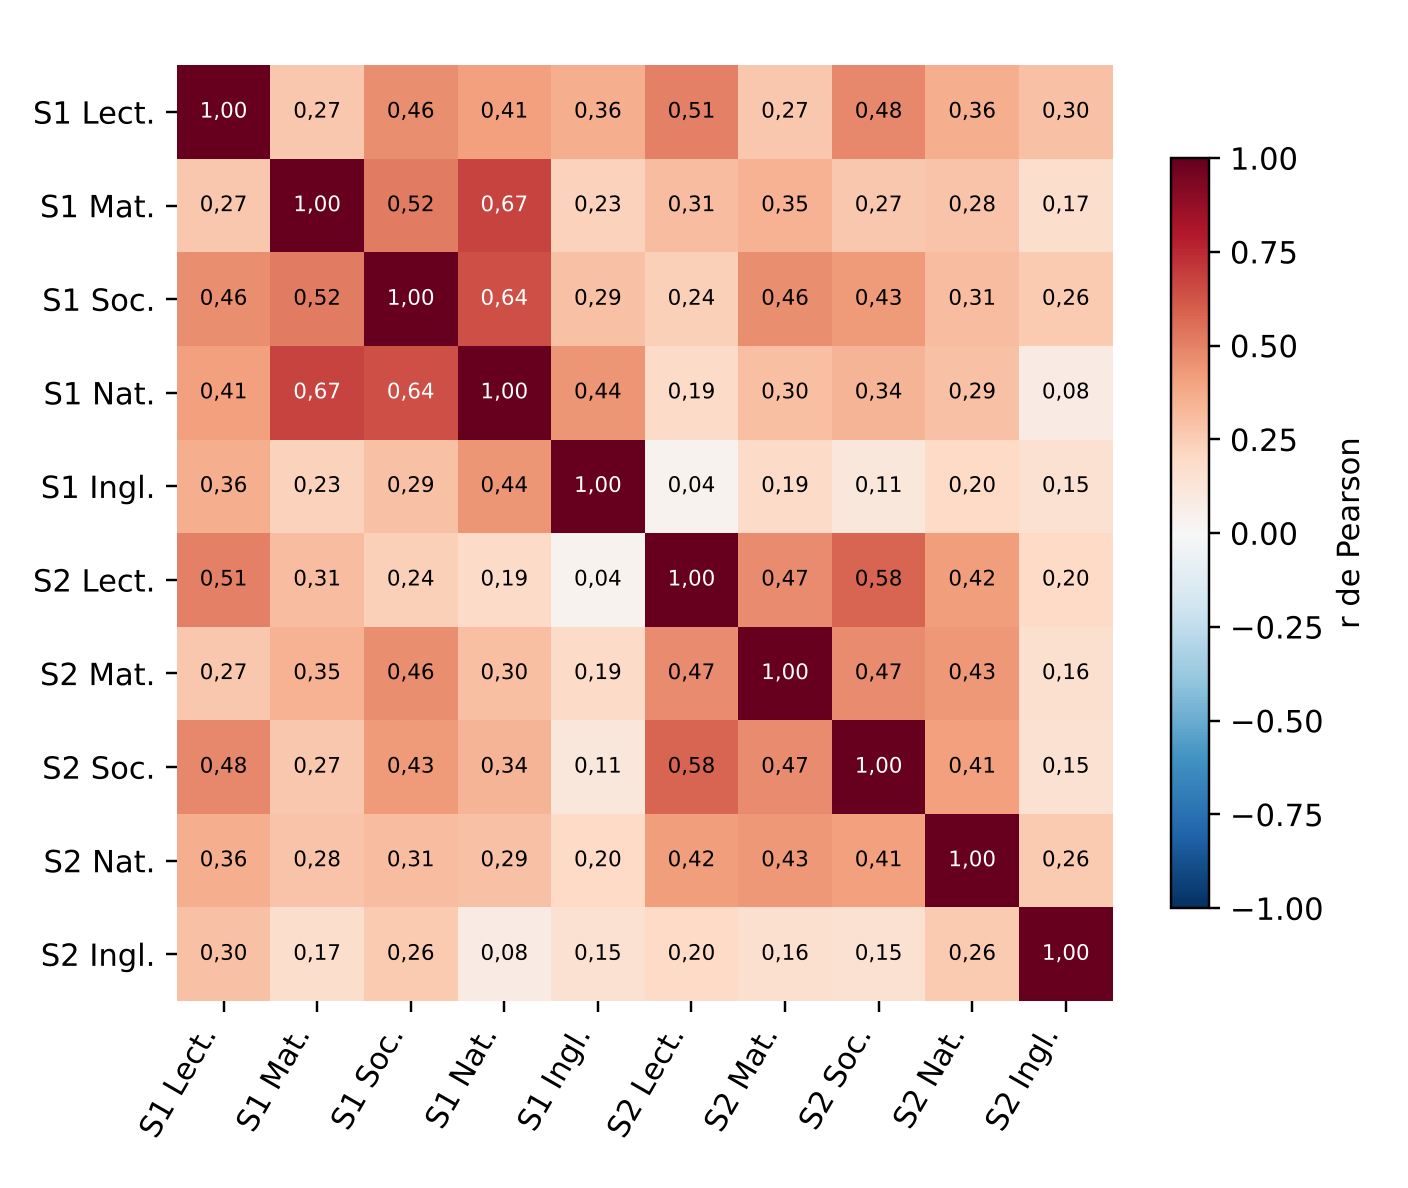
\includegraphics[width=0.95\columnwidth]{img/figA1_correlacion_areas.png}
    \caption{Correlación entre las diez áreas de los simulacros, calculada solo con Train (cohorte 2025).}
    \label{fig:colinealidad}
\end{figure}

\subsection*{A-3. Preprocesamiento dentro de \textit{pipelines}}

Todo paso que aprende de los datos se ajustó solo con Train, dentro de un \textit{pipeline} de scikit-learn \parencite{pedregosa2011scikit}:

\begin{itemize}
    \item \textit{Imputación:} SimpleImputer (mediana) en el análisis principal e IterativeImputer en el de sensibilidad. Para este último, los valores que la base de modelado tenía imputados se volvieron a marcar como faltantes y se imputaron dentro del \textit{pipeline}, de modo que la imputación de Test usa solo lo aprendido en Train \parencite{vanbuuren2018flexible}.
    \item \textit{Escalado:} StandardScaler, ajustado con la media y la desviación de Train.
    \item \textit{Validación cruzada interna:} en cada pliegue el \textit{pipeline} completo se reajusta, así que el pliegue de validación tampoco influye en la imputación ni en el escalado.
\end{itemize}

\section*{Anexo B. Implementación y traducción a decisiones}
\markboth{Anexo B}{Anexo B}
\setcounter{table}{0}\renewcommand{\thetable}{B-\Roman{table}}
\setcounter{figure}{0}\renewcommand{\thefigure}{B\arabic{figure}}

\subsection*{B-1. Del modelo a la probabilidad}

La regresión logística con el promedio de S1 y S2 devuelve, para cada estudiante, la probabilidad de terminar en el cuartil inferior. Esa probabilidad no es todavía una decisión: hay que elegir a partir de qué valor se asigna refuerzo.

\subsection*{B-2. Selección de umbrales según el costo de equivocarse}

Se asumió que dejar sin refuerzo a un estudiante en riesgo (falso negativo) es tres veces más costoso que reforzar a uno que no lo necesitaba (falso positivo). Con las probabilidades fuera de pliegue de Train se calcularon dos umbrales (figura~\ref{fig:umbrales}):

\begin{itemize}
    \item \textit{Umbral de decisión} (\textit{p}~=~0,23): minimiza el costo esperado con la relación 3 a 1. Decide si el estudiante recibe o no refuerzo.
    \item \textit{Umbral de prioridad alta} (\textit{p}~=~0,38): minimiza el total de errores con costos iguales. Es más exigente y separa a quienes necesitan refuerzo intensivo.
\end{itemize}

\begin{figure}[!t]
    \centering
    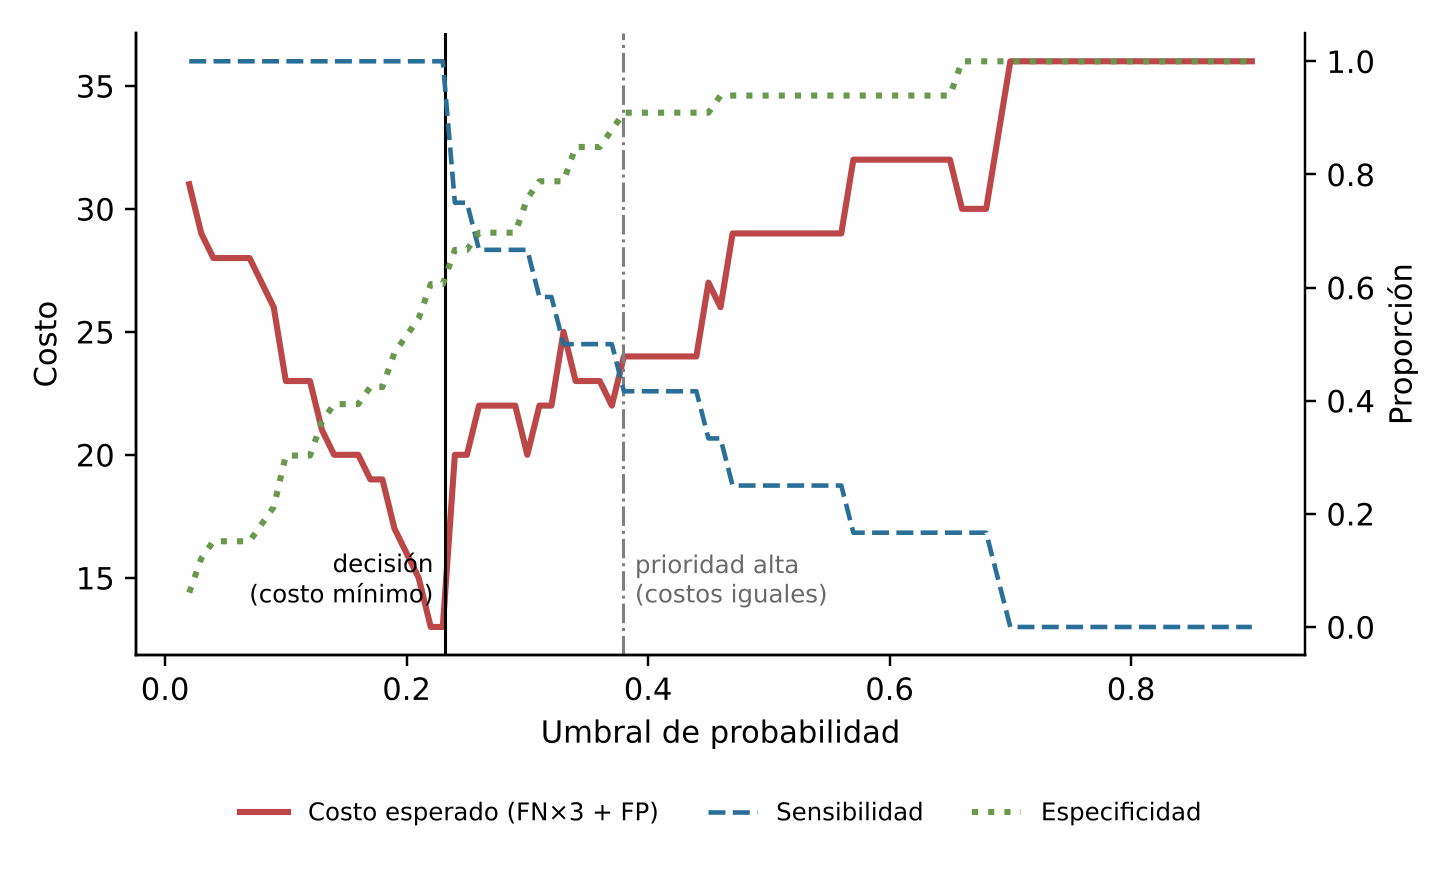
\includegraphics[width=\columnwidth]{img/figB1_umbrales_costo.png}
    \caption{Costo esperado, sensibilidad y especificidad según el umbral (Train, probabilidades fuera de pliegue).}
    \label{fig:umbrales}
\end{figure}

\subsection*{B-3. Matriz de confusión en Test}

\begin{figure}[!t]
    \centering
    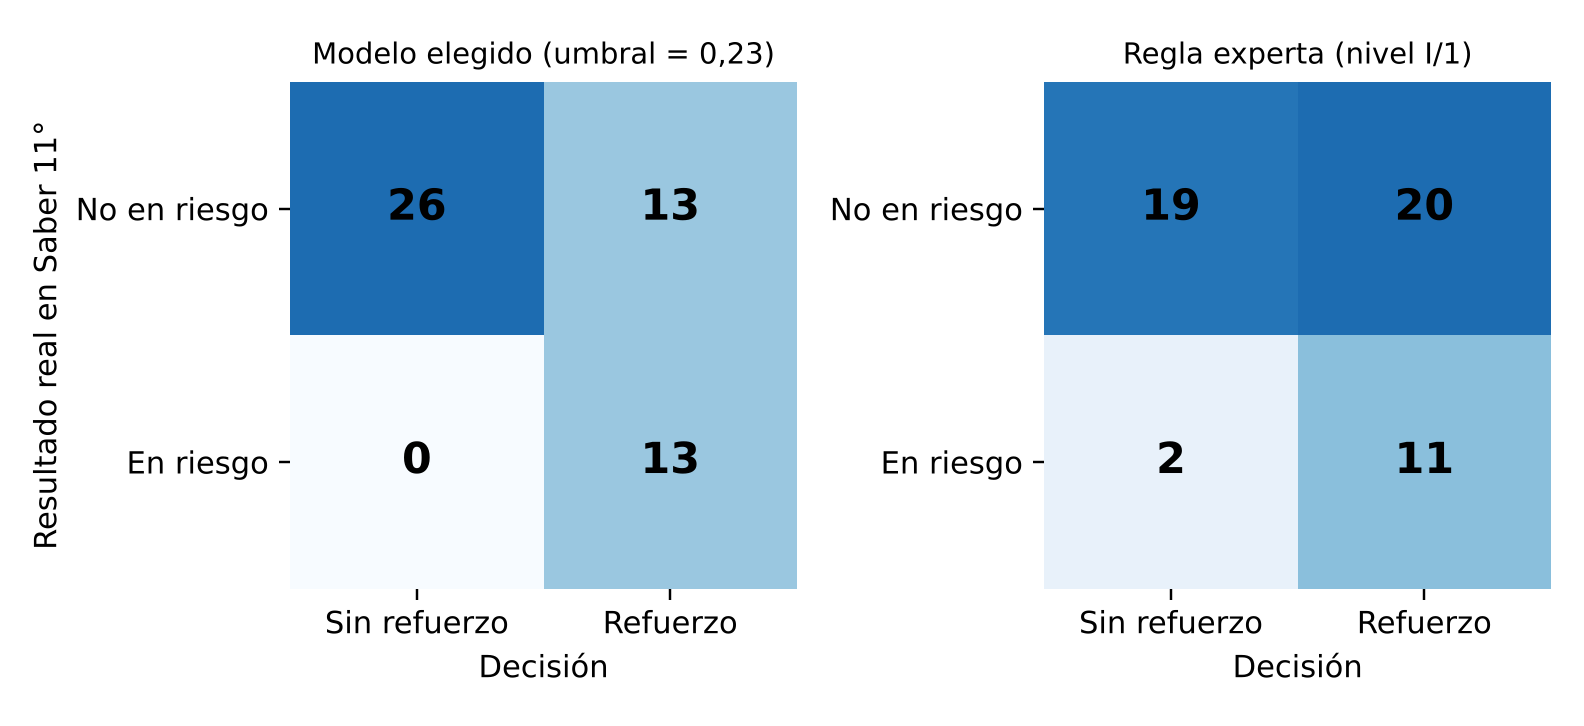
\includegraphics[width=\columnwidth]{img/figB2_matrices_confusion.png}
    \caption{Matrices de confusión en Test (cohorte 2026): modelo elegido frente a la regla de la empresa.}
    \label{fig:confusion}
\end{figure}

Con el umbral de decisión, el modelo asignó refuerzo a 26 de los 52 estudiantes de 2026. Ese grupo incluye a los 13 que terminaron en el cuartil inferior (ningún falso negativo) y a 13 que no lo necesitaban. La regla de la empresa (nivel I/1) habría asignado refuerzo a 31 estudiantes, dejado por fuera a 2 en riesgo y marcado a 20 que no lo estaban (figura~\ref{fig:confusion}). En términos prácticos, el modelo protege a todos los estudiantes en riesgo con 5 cupos de refuerzo menos.

\subsection*{B-4. Regla de tres prioridades}

Como el modelo usa una sola variable, cada umbral de probabilidad equivale a un puntaje del promedio de S1 y S2. Así, la regla se puede aplicar con una hoja de cálculo o a mano (tabla~\ref{tb:prioridades}).

\begin{table}[!t]
\centering
\footnotesize
\renewcommand{\arraystretch}{1.15}
\begin{tabularx}{\columnwidth}{@{}l c c >{\centering\arraybackslash}X c@{}}
\toprule
\textbf{Prioridad} & \textbf{\shortstack{Promedio\\$\bar{S}$}} & \textbf{\shortstack{Estu-\\diantes}} & \textbf{\shortstack{En el cuartil\\inferior}} & \textbf{\shortstack{SB11\\medio}} \\
\midrule
Alta  & $\leq 182{,}5$    & 17 & 9 (53\,\%) & 203,1 \\
Media & $(182{,}5;\ 202{,}4]$    & 9  & 4 (44\,\%) & 217,0 \\
Baja  & $> 202{,}4$       & 26 & 0 (0\,\%)  & 261,2 \\
\bottomrule
\end{tabularx}
\caption{Prioridades en Test (cohorte 2026) según el promedio de S1 y S2.}
\label{tb:prioridades}
\end{table}

La ruta de uso queda así: después de S1 se emite una alerta preliminar; después de S2 se calcula el promedio y se asigna la prioridad; la inasistencia a cualquiera de los simulacros sube la prioridad un nivel; y, cuando llega el resultado oficial, el modelo se reentrena sumando la nueva cohorte.

\section*{Anexo C. Métricas, línea base y sobreajuste}
\markboth{Anexo C}{Anexo C}
\setcounter{table}{0}\renewcommand{\thetable}{C-\Roman{table}}
\setcounter{figure}{0}\renewcommand{\thefigure}{C\arabic{figure}}

\subsection*{C-1. Regresión: Train frente a Test}

\begin{table*}[!t]
\centering
\small
\begin{tabular}{@{}lccccccc@{}}
\toprule
\textbf{Modelo} & \textbf{MAE Train} & \textbf{MAE Test} & \textbf{Brecha} & \textbf{RMSE Test} & \textbf{$\boldsymbol{R^2}$ Train} & \textbf{$\boldsymbol{R^2}$ Test} & \textbf{MAE inverso} \\
\midrule
Línea base (media) & 36,2 & 27,7 & $-8{,}5$ & 33,6 & 0,00 & 0,00 & 36,1 \\
Regla experta (S2 bruto) & 30,6 & 33,5 & 2,8 & 43,6 & 0,27 & $-0{,}69$ & 30,6 \\
Lineal $\cdot$ promedio S1-S2 & 19,3 & 18,1 & $-1{,}2$ & 22,4 & 0,63 & 0,55 & 23,1 \\
Ridge $\cdot$ 10 áreas & 17,6 & 16,4 & $-1{,}2$ & 21,7 & 0,69 & 0,58 & 23,7 \\
Random Forest $\cdot$ 10 áreas & 11,1 & 15,2 & 4,1 & 19,8 & 0,88 & 0,65 & 26,0 \\
\bottomrule
\end{tabular}
\caption{Regresión de SB11\_GLOBAL. Train~=~2025, Test~=~2026; última columna: sentido inverso (Train 2026~$\rightarrow$~Test 2025).}
\label{tb:regresion}
\end{table*}

Los valores de la tabla~\ref{tb:regresion} se resumen en la figura~\ref{fig:mae}.

\begin{figure}[!t]
    \centering
    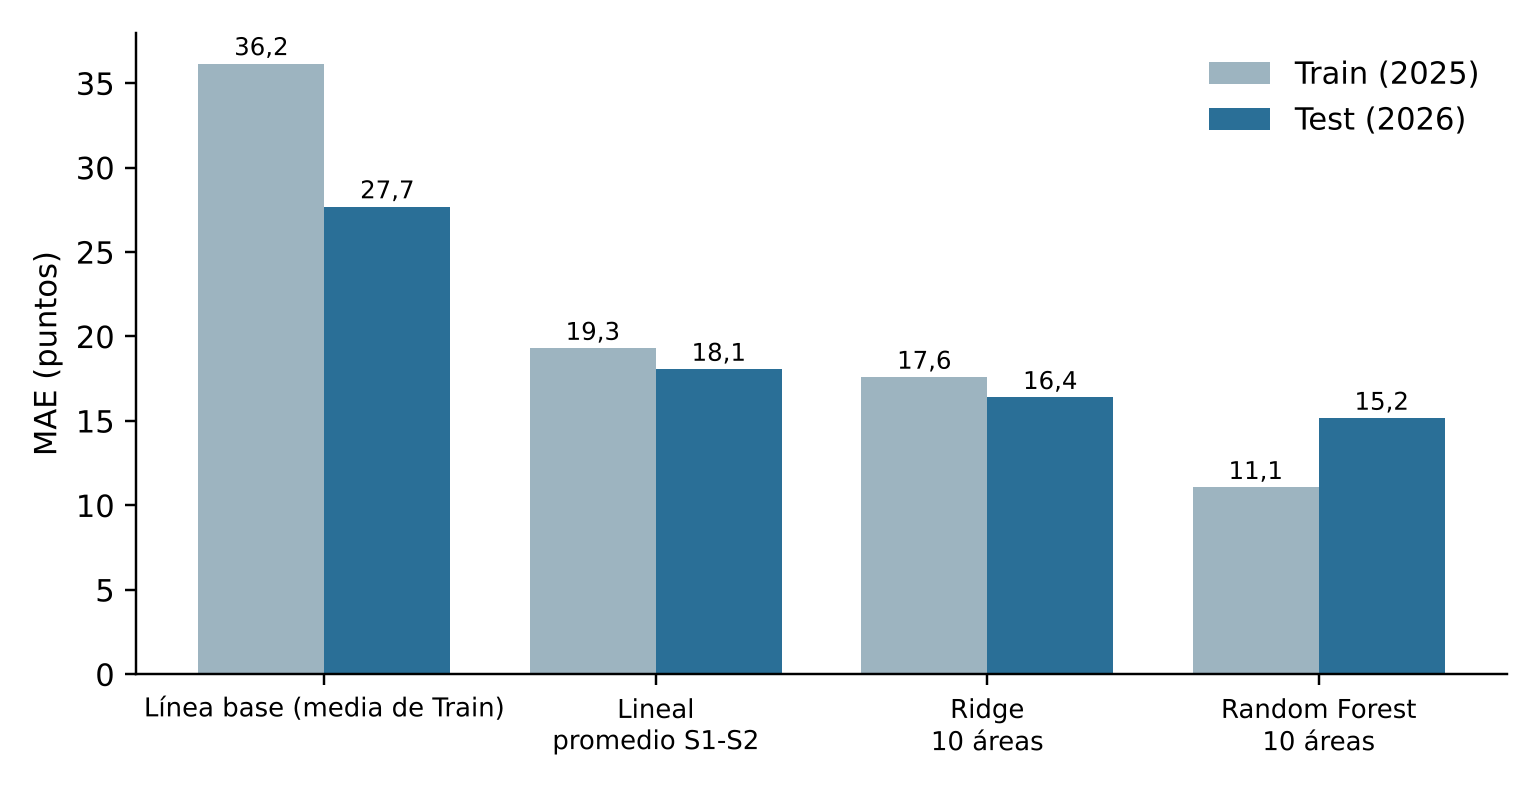
\includegraphics[width=\columnwidth]{img/figC1_mae_train_test.png}
    \caption{Error medio absoluto en Train y en Test. Una brecha positiva indica sobreajuste.}
    \label{fig:mae}
\end{figure}

El modelo lineal y Ridge tienen errores parecidos en Train y en Test, lo que indica que no sobreajustan (figura~\ref{fig:mae}). Random Forest obtiene el menor error en Train (11,1), pero en Test su MAE sube 4,1 puntos y, al invertir los años, es el más alto de los modelos entrenados (26,0). Ridge reduce el MAE del lineal en 1,7 puntos en Test (16,4 frente a 18,1), pero lo aumenta en 0,6 al invertir los años (23,7 frente a 23,1); no cumple, por tanto, el criterio de mejorar en al menos dos puntos en ambas direcciones. Por estas razones se conserva el modelo lineal.

\subsection*{C-2. Clasificación: Train frente a Test}

\begin{table*}[!t]
\centering
\small
\begin{tabular}{@{}lcccccccc@{}}
\toprule
\textbf{Modelo} & \textbf{AUC Train} & \textbf{AUC Test} & \textbf{AUC-PR} & \textbf{Exact. bal.} & \textbf{Sens.} & \textbf{Espec.} & \textbf{Prec.} & \textbf{F1} \\
\midrule
Línea base (mayoritaria) & 0,50 & 0,50 & 0,25 & 0,50 & 0,00 & 1,00 & 0,00 & 0,00 \\
Regla experta (I/1) & 0,71 & 0,67 & 0,34 & 0,67 & 0,85 & 0,49 & 0,35 & 0,50 \\
Logística $\cdot$ promedio & 0,82 & 0,87 & 0,62 & 0,83 & 1,00 & 0,67 & 0,50 & 0,67 \\
Logística L2 $\cdot$ 10 áreas & 0,86 & 0,87 & 0,63 & 0,81 & 0,92 & 0,69 & 0,50 & 0,65 \\
Random Forest $\cdot$ 10 áreas & 0,97 & 0,87 & 0,73 & 0,74 & 0,77 & 0,72 & 0,48 & 0,59 \\
\bottomrule
\end{tabular}
\caption{Clasificación del riesgo (cuartil inferior). Métricas de Test con el umbral elegido en Train.}
\label{tb:clasificacion}
\end{table*}

La tabla~\ref{tb:clasificacion} compara los clasificadores y la figura~\ref{fig:roc} muestra sus curvas ROC.

\begin{figure}[!t]
    \centering
    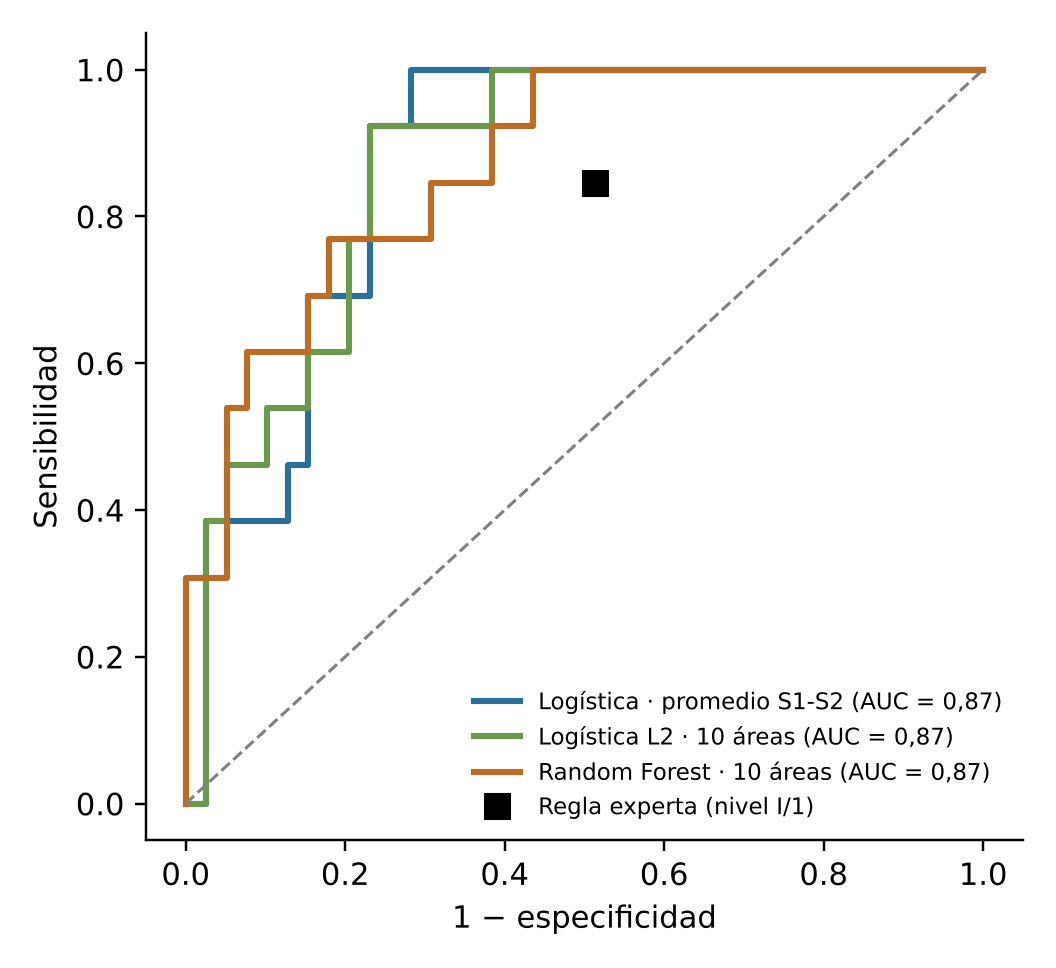
\includegraphics[width=0.9\columnwidth]{img/figC2_curvas_roc.png}
    \caption{Curvas ROC en Test (cohorte 2026) y punto de operación de la regla de la empresa.}
    \label{fig:roc}
\end{figure}

\subsection*{C-3. Lectura de los resultados}

\begin{itemize}
    \item \textit{Métricas adecuadas.} La línea base alcanza la misma exactitud que el modelo elegido (0,75) sin detectar a ningún estudiante en riesgo. Por eso la elección se basa en la sensibilidad, la exactitud balanceada y las áreas bajo las curvas \parencite{saito2015precision}.
    \item \textit{Sobreajuste.} La logística con el promedio no sobreajusta: su AUC es de 0,82 en Train y de 0,87 en Test. Random Forest, en cambio, baja de 0,97 en Train a 0,87 en Test.
    \item \textit{Comparación con la regla experta.} El modelo elegido tiene una sensibilidad de 1,00 frente a 0,85, una especificidad de 0,67 frente a 0,49 y una precisión de 0,50 frente a 0,35 (figura~\ref{fig:roc}), y reduce los falsos positivos de 20 a 13. Como los intervalos individuales se solapan, la diferencia se respalda con la prueba pareada de McNemar (\textit{p}~=~0,004).
    \item \textit{Robustez.} Al invertir los años, la logística con el promedio obtiene un AUC de 0,82. Con los 112 estudiantes, imputando dentro del \textit{pipeline}, el AUC es de 0,86, con una sensibilidad de 0,86 y una especificidad de 0,76.
\end{itemize}

\subsection*{C-4. Reproducibilidad}

Las cifras de este documento se generan con el cuaderno \texttt{Anexo\_tecnico\_modelo\_Saber11.ipynb}, que lee las dos bases de modelado anonimizadas y fija la semilla aleatoria en 2025. Los intervalos de confianza, el \textit{bootstrap} y la prueba de McNemar se calculan con el script \texttt{incertidumbre\_bootstrap\_mcnemar.py}, que reproduce las predicciones de cada estudiante a partir de las mismas bases, y los coeficientes de la sección IV-B, con \texttt{interpretabilidad\_coeficientes.py}.

\end{document}
